\section{Question 3}

\paragraph{\textbf{System architecture}}
The diagram in Fig.\ref{fig:q3_diagram} summarizes our final system architecture for Question 3.

\begin{figure}[!h]
    \centering
    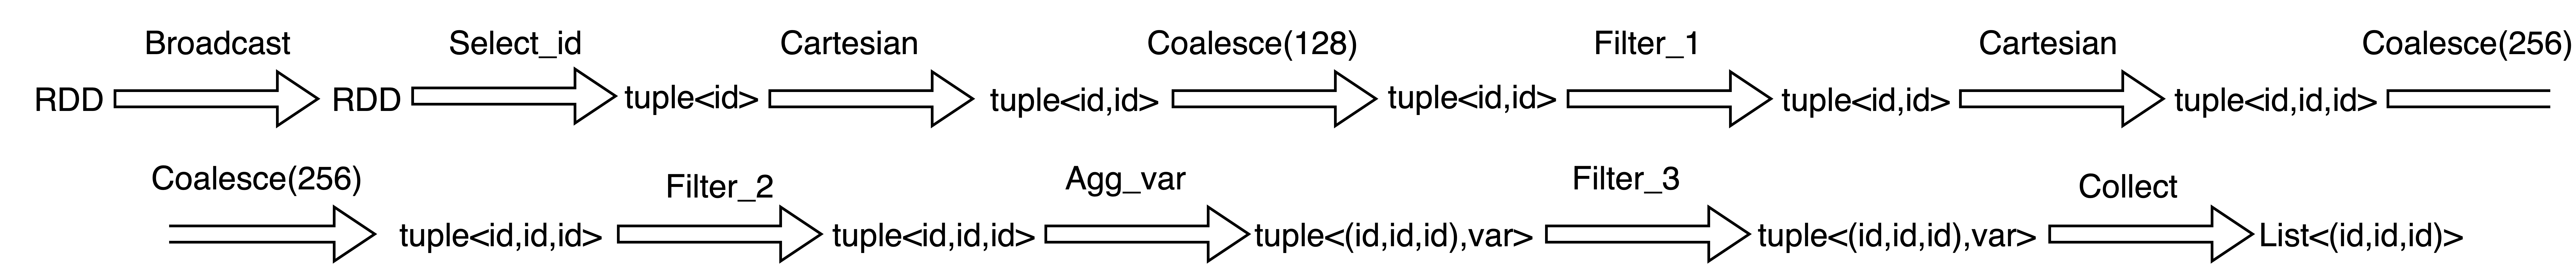
\includegraphics[width=.95\linewidth]{../assets/images/q3_diagram.png}
    \caption{Brief description of system architecture for Q3}
    \label{fig:q3_diagram}
\end{figure}

\begin{itemize}
    \item \mintinline{python}{Broadcast}: broadcasts a $<\textrm{id}, \textrm{vector}>$ map over the worker nodes.
    \item \mintinline{python}{Select_id}: filters the RDD such that the \mintinline{python}{.cartesian()} will be computed only on ids.
    \item \mintinline{python}{Cartesian}: performs the cartesian product of the RDD with itself; outputs a new RDD of length \mintinline{python}{len(rdd)}$^{2}$.
    \item \mintinline{python}{Coalesce(number)}: returns a new RDD with at most \mintinline{python}{numPartitions} number of partitions.
    \item \mintinline{python}{Filter_1}: filters out all tuples where the first element is greater than or equal to the second, preventing duplicates.
    \item \mintinline{python}{Filter_2}: filters out all tuples where the second element is greater than or equal to the third, preventing duplicates.
    \item \mintinline{python}{Agg_var}: gets the vectors associated with the keys in the tuples from the broadcast variable, calculates the aggregate variance, adds 1 to the accumulator if it's less than or equal to 410, and returns a pair with the keys tuple and the variance. 
    \item \mintinline{python}{Filter_3}: filters out all variances greater than 20.
    \item \mintinline{python}{Collect}: returns a Python list with all the elements in the RDD.
\end{itemize}

\paragraph{\textbf{Performances and optimizations}}
The execution time of Q3 on the cluster was \textbf{910.05 seconds}. In the following, we summarize the most important optimization tricks we leveraged to obtain our results. The impact of each optimization tricks is summarized in Tab.\ref{tab:q3_local_optimisations} and Tab.\ref{tab:q3_server_optimisations}.

\begin{itemize}
    \item We use \mintinline{python}{numpy.ndarray}s of 16 bits of precision to represent the values of the vectors (see Sec.\ref{sec:q2}).
    \item We broadcast the vector map to reduce the network transfer during the shuffle phases (see Sec.\ref{sec:q2}).
    \item We used the \mintinline{python}{.coalesce()} API to reduce the number of partitions after the \mintinline{python}{.cartesian()} operations (see Sec.\ref{sec:q2}).
    \item We used the \mintinline{python}{.Accumulator()} API during the variance computation: this allowed us to filter out the \(\tau \leq 20\) triples while still retaining in the accumulator the amount of triples with \(\tau \leq 410\).
\end{itemize}

\begin{table}[H]
    \begin{minipage}{.45\textwidth}
    \centering
    \begin{tabular}{l c}
    \toprule
    \textbf{Optimization} & \textbf{Execution time} \\
    \midrule
    All            & 30.59s     \\
    No numpy       & 2940.19s   \\
    No broadcast   & 185.30s    \\ 
    No accumulator & 36.44s     \\
    No coalesce    & 131.46s    \\
    \bottomrule
\end{tabular}
\caption{Impact of optimizations tricks on the dataset of size 250x10000, ran locally.}
\label{tab:q3_local_optimisations}
    \end{minipage}
    \hfill
    \begin{minipage}{.5\textwidth}
        \centering
        \begin{tabular}{l c}
    \toprule
    \textbf{Partitions} & \textbf{Execution time} \\
    \midrule
    64-128-256     & 910.05s    \\ 
    128-256-512    & 946.79s    \\ 
    125-250-500    & 969.51s    \\ 
    64-64-128      & 1005.65s   \\
    25-50-100      & 1097.70s   \\
    64-64-64       & 1122.74s   \\
    128-128-128    & 1162.01s   \\
    \bottomrule
\end{tabular}
\caption{Impact of partition combinations on the dataset of size 1000x10000, ran on the server.}
\label{tab:q3_server_optimisations}
    \end{minipage}
\end{table}

Besides the aforementioned, we have tried a variety of optimization strategies; even though they were discarded, some of them are still worth reporting, as a considerable amount of effort was put into them and they can still be useful in other scenarios.
\begin{itemize}
    \item We tried to pre-process the RDD, to obtain the mean of each row before the variance computation and then used this mean as input for the \mintinline{python}{statistics.pvariance()} function. This allowed us to save some time for all the aggregate variance computation. We discarded this technique in favor of the usage of \mintinline{python}{numpy.var()}.
    \item A thing we tried instead of using an accumulator, was filtering out all triples with \(\tau \leq 410\) and caching these. Using this cache we could then both count these triples and get the triples with \(\tau \leq 20\) by filtering again. It turned out that using the accumulator was slightly faster.
\end{itemize}

\paragraph{\textbf{Discussion on Q3 vs Q2}}
\begin{wrapfigure}{r}{0.44\textwidth}
  \centering
  \begin{tabular}{l r r c}
    \toprule
    {} & \textbf{Q2 code} & \textbf{Q3 code} \\
    \midrule
    Results $\tau = 20$ & 2
    % 2%, [ARSR-JIIT-JY1T], [CFIL-D4U2-OE4G] 
    & 10  \\
    Results $\tau = 420$ & 2%, [ARSR-JIIT-JY1T], [CFIL-D4U2-OE4G]
    & 10  \\
    \midrule
    Execution time & 237.11 & 42.35&  \\
    \bottomrule
\end{tabular}
\makeatletter\def\@captype{table}\makeatother% "Change float to table"
\caption{Comparison between Q2 code and Q3 code on the same dataset (250 vectors).}
\label{tab:q2-vs-q3}
\end{wrapfigure}
We ran the code for \emph{Question 3} on the dataset generated for \emph{Question 2} and we found out that the results are the same (they are summarized in Tab.\ref{tab:q2-vs-q3}).

While the two implementations produce the same results, the execution time of the code of Q3 is significantly smaller than the execution time of Q2. It is not trivial to understand the reason behind such behavior since the overall approach is comparable in its core steps and all the main optimization techniques were employed in both implementations. 

One possible reason can be the different usage of \mintinline{python}{.coalesce()} and \mintinline{python}{.repartition()}. In the code of Q2, we employ one \mintinline{python}{.repartition()} on the dataframe with only the keys, before then doubling the partition count after each \mintinline{python}{.crossJoin()}; meanwhile, in Q3 we also use \mintinline{python}{.coalesce()} twice, once after every \mintinline{python}{.cartesian()} call (after the first we reduce the partitions to 128, and after the second to 256), while the repartition is inherited from the initial RDD creation. It may be the case that the configuration of partitions is suboptimal and, subsequently, our implementation for Q2 is not parallelizing enough to leverage the computing power of the cluster, or conversely, we are parallelizing too much. However, we have not found a better combination of partition counts: such values for the partitions are not trivial for us to determine and require a lot of trial and error and empirical evaluation; hence, we still believe that our solution for Q2 is valuable.

One other reason could be that our implementation of Q3 only queries 2 values (\(\tau = 20\) and \(\tau = 410\)), while the solution for Q2 queries 5 values. However, since most of the time is taken by the combinations and aggregate variances computations, it is unlikely that this is the reason behind the lower performances of Q2.

Ultimately, the \mintinline{python}{DataFrame} API of SparkSQL might be inherently slower than the usage of plain Spark, or at least in our use-case, since the former is a library built on top of the Spark Core. In particular, the combination of a large user-defined function with SparkSQL might slow the overall execution down.
